\documentclass[12pt]{article}
\author{Michael Vu}
\title{Numerical Analysis HW 5}
\usepackage{pdfsync} %This package allows for some communication between your pdf viewer and your latex editor, so that you can double click on a line in the pdf, for instance, and it will jump to the corresponding line in your latex code.

\usepackage{amssymb, amsmath, graphicx,amsthm} %these are standard packages that I pretty much always use.

\usepackage{bm,stmaryrd,verbatim,color,amsbsy}
%\usepackage{showkeys}  %If you have trouble remembering what you labeled your equations, you can uncomment this package, and temporarily see the labels displayed.
\usepackage{epstopdf} %Since I use Maple sometimes to make figures, and I get it to output eps files, I use this package so that eps files can be inputted into my documents. 
%Mathematica has the ability to output figures as pdfs, which are handled automatically with the graphicx package enabled.

\usepackage[normalem]{ulem} %this is a package that lets you underline, but mostly I like the \sout command for striking out.

\usepackage{color} %this package lets us change the color of your font by writing something like {\color[rgb]{1,0,0} This would be red}.




\def\red #1{{\color[rgb]{1, 0,0}#1}} %To make things easy on myself, I define a simpler function like this, so I can write \red{This would be red} instead of the above babble.

\newtheorem{theorem}{Theorem}[section]
\newtheorem{lemma}[theorem]{Lemma}
\newtheorem{proposition}[theorem]{Proposition}
\newtheorem{corollary}[theorem]{Corollary} %These define theorem like environments.

\newenvironment{definition}[1][Definition]{\begin{trivlist}
\item[\hskip \labelsep {\bfseries #1}]}{\end{trivlist}}
\newenvironment{example}[1][Example]{\begin{trivlist}
\item[\hskip \labelsep {\bfseries #1}]}{\end{trivlist}}
\newenvironment{remark}[1][Remark]{\begin{trivlist}
\item[\hskip \labelsep {\bfseries #1}]}{\end{trivlist}} %These define various other types of math environments: definition, example, and remarks.

\newcommand{\ph}{\varphi}






\bibliographystyle{plain}


%Some common or not so common symbols that I wanted shortcuts for.
\newcommand{\eps}{\varepsilon}
\newcommand{\ddt}{\frac{\mbox{d}}{\mbox{d}t}}
\newcommand{\dA}{\,\mbox{d}A}
\newcommand{\dv}{\,\mbox{d}v}
\def\dx{\, \mbox{d} x}
\newcommand{\ds}{\,\mbox{d}s}
\newcommand{\dz}{\,\mbox{d}z}
\def\dzeta{\,\mbox{d}\zeta}
\newcommand{\dl}{\,\mbox{d}l}
\renewcommand{\div}{\mbox{ div}}
\newcommand{\grad}{\mbox{ grad }}




%bold letters usually used to denote vectors matrices.
\def\bfa{\mathbf{a}}
\def\bfA{\mathbf{A}}
\def\bfb{\mathbf{b}}
\def\bfB{\mathbf{B}}
\def\bfc{\mathbf{c}}
\def\bfC{\mathbf{C}}
\def\bfd{\mathbf{d}}
\def\bfD{\mathbf{D}}
\def\bfe{\mathbf{e}}
\def\bfE{\mathbf{E}}
\def\bff{\mathbf{f}}
\def\bfF{\mathbf{F}}
\def\bfg{\mathbf{g}}
\def\bfG{\mathbf{G}}
\def\bfh{\mathbf{h}}
\def\bfH{\mathbf{H}}
\def\bfi{\mathbf{i}}
\def\bfI{\mathbf{I}}
\def\bfj{\mathbf{j}}
\def\bfJ{\mathbf{J}}
\def\bfk{\mathbf{k}}
\def\bfK{\mathbf{K}}
\def\bfl{\mathbf{l}}
\def\bfL{\mathbf{L}}
\def\bfm{\mathbf{m}}
\def\bfM{\mathbf{M}}
\def\bfn{\mathbf{n}}
\def\bfN{\mathbf{N}}
\def\bfo{\mathbf{o}}
\def\bfO{\mathbf{O}}
\def\bfp{\mathbf{p}}
\def\bfP{\mathbf{P}}
\def\bfq{\mathbf{q}}
\def\bfQ{\mathbf{Q}}
\def\bfr{\mathbf{r}}
\def\bfR{\mathbf{R}}
\def\bfs{\mathbf{s}}
\def\bfS{\mathbf{S}}
\def\bft{\mathbf{t}}
\def\bfT{\mathbf{T}}
\def\bfu{\mathbf{u}}
\def\bfU{\mathbf{U}}
\def\bfv{\mathbf{v}}
\def\bfV{\mathbf{V}}
\def\bfw{\mathbf{w}}
\def\bfW{\mathbf{W}}
\def\bfx{\mathbf{x}}
\def\bfX{\mathbf{X}}
\def\bfy{\mathbf{y}}
\def\bfY{\mathbf{Y}}
\def\bfz{\mathbf{z}}
\def\bfZ{\mathbf{Z}}



%``Blackboard bold" letters \bbC is used for the complex plane, \bbN
\def\bba{\mathbb{a}}
\def\bbA{\mathbb{A}}
\def\bbb{\mathbb{b}}
\def\bbB{\mathbb{B}}
\def\bbc{\mathbb{c}}
\def\bbC{\mathbb{C}}
\def\bbd{\mathbb{d}}
\def\bbD{\mathbb{D}}
\def\bbe{\mathbb{e}}
\def\bbE{\mathbb{E}}
\def\bbf{\mathbb{f}}
\def\bbF{\mathbb{F}}
\def\bbg{\mathbb{g}}
\def\bbG{\mathbb{G}}
\def\bbh{\mathbb{h}}
\def\bbH{\mathbb{H}}
\def\bbi{\mathbb{i}}
\def\bbI{\mathbb{I}}
\def\bbj{\mathbb{j}}
\def\bbJ{\mathbb{J}}
\def\bbk{\mathbb{k}}
\def\bbK{\mathbb{K}}
\def\bbl{\mathbb{l}}
\def\bbL{\mathbb{L}}
\def\bbm{\mathbb{m}}
\def\bbM{\mathbb{M}}
\def\bbn{\mathbb{n}}
\def\bbN{\mathbb{N}}
\def\bbo{\mathbb{o}}
\def\bbO{\mathbb{O}}
\def\bbp{\mathbb{p}}
\def\bbP{\mathbb{P}}
\def\bbq{\mathbb{q}}
\def\bbQ{\mathbb{Q}}
\def\bbr{\mathbb{r}}
\def\bbR{\mathbb{R}}
\def\bbs{\mathbb{s}}
\def\bbS{\mathbb{S}}
\def\bbt{\mathbb{t}}
\def\bbT{\mathbb{T}}
\def\bbu{\mathbb{u}}
\def\bbU{\mathbb{U}}
\def\bbv{\mathbb{v}}
\def\bbV{\mathbb{V}}
\def\bbw{\mathbb{w}}
\def\bbW{\mathbb{W}}
\def\bbx{\mathbb{x}}
\def\bbX{\mathbb{X}}
\def\bby{\mathbb{y}}
\def\bbY{\mathbb{Y}}
\def\bbz{\mathbb{z}}
\def\bbZ{\mathbb{Z}}

\def\ca{\mathcal{a}}
\def\cA{\mathcal{A}}
\def\cb{\mathcal{b}}
\def\cB{\mathcal{B}}
\def\cc{\mathcal{c}}
\def\cC{\mathcal{C}}
\def\cd{\mathcal{d}}
\def\cD{\mathcal{D}}
\def\ce{\mathcal{e}}
\def\cE{\mathcal{E}}
\def\cf{\mathcal{f}}
\def\cF{\mathcal{F}}
\def\cg{\mathcal{g}}
\def\cG{\mathcal{G}}
\def\ch{\mathcal{h}}
\def\cH{\mathcal{H}}
\def\ci{\mathcal{i}}
\def\cI{\mathcal{I}}
\def\cj{\mathcal{j}}
\def\cJ{\mathcal{J}}
\def\ck{\mathcal{k}}
\def\cK{\mathcal{K}}
\def\cl{\mathcal{l}}
\def\cL{\mathcal{L}}
\def\cm{\mathcal{m}}
\def\cM{\mathcal{M}}
\def\cn{\mathcal{n}}
\def\cN{\mathcal{N}}
\def\co{\mathcal{o}}
\def\cO{\mathcal{O}}
\def\cp{\mathcal{p}}
\def\cP{\mathcal{P}}
\def\cq{\mathcal{q}}
\def\cQ{\mathcal{Q}}
\def\calr{\mathcal{r}}
\def\cR{\mathcal{R}}
\def\cs{\mathcal{s}}
\def\cS{\mathcal{S}}
\def\ct{\mathcal{t}}
\def\cT{\mathcal{T}}
\def\cu{\mathcal{u}}
\def\cU{\mathcal{U}}
\def\cv{\mathcal{v}}
\def\cV{\mathcal{V}}
\def\cw{\mathcal{w}}
\def\cW{\mathcal{W}}
\def\cx{\mathcal{x}}
\def\cX{\mathcal{X}}
\def\cy{\mathcal{y}}
\def\cY{\mathcal{Y}}
\def\cz{\mathcal{z}}
\def\cZ{\mathcal{Z}}

%Some operators that I wanted displayed in a similar font as you would want sin and cos functions (by the way, those can be called up by using \sin,\cos,\log,\ln, \tan,\exp,\sec,\csc,\sinh,\cosh,\tanh, there are probably more.
\DeclareMathOperator*{\sgn}{sgn}
\DeclareMathOperator*{\spn}{span}
\DeclareMathOperator*{\coker}{coker}
\DeclareMathOperator*{\Id}{Id}
\DeclareMathOperator*{\D}{D}
\def\RR{\mathbb{R}}

%more symbols that I wanted extra short commands for
\newcommand{\be}{\mathbf{e}}
\renewcommand{\L}{\Lambda}
\newcommand{\vs}{\varsigma}
\newcommand{\al}{\alpha}
\newcommand{\s}{\sigma}
\renewcommand{\k}{\kappa}
\renewcommand{\t}{\theta}
\newcommand{\w}{\omega}


%some bold greek letters.
\def\bfeta{\boldsymbol{\eta}}
\def\bfxi{\boldsymbol{\xi}}
\def\bfrho{\boldsymbol{\rho}}
\def\bfth{\boldsymbol{\t}}
\def\bflam{\boldsymbol{\lambda}}
\def\bfTh{\boldsymbol{\Theta}}
\def\bfnu{\boldsymbol{\nu}}

\newcommand{\drho}{\,{\rm d} \rho}
\newcommand{\dth}{\,{\rm d} \t}
\newcommand{\tilu}{\tilde{u}}
\newcommand{\vt}{\vartheta}


\begin{document}

\maketitle 

\textbf{Problem 1.} Using a divided difference program, I recreated the table 3.9 from our textbook with this code:

\begin{verbatim}
program hw5pr1
implicit none
integer :: n, i, k
double precision :: x(0:4), f(0:4), a(0:4)
double precision :: t(0:4, 0:4), top, bottom

x(0) = 1.0d0
x(1) = 1.3d0
x(2) = 1.6d0
x(3) = 1.9d0
x(4) = 2.2d0

f(0) = 0.7651977d0
f(1) = 0.6200860d0
f(2) = 0.4554022d0
f(3) = 0.2818186d0
f(4) = 0.1103623d0

do i = 0, 4 
	t(i, 0) = f(i)
end do

do k = 1, 4 
	do i = k, 4 
		top = t(i, k-1) - t(i-1, k-1)
		bottom = x(i) - x(i-k)
		t(i, k) = top / bottom
	end do
end do

write(*,6) t(0,0)
write(*,6) t(1,0:1)
write(*,6) t(2,0:2)
write(*,6) t(3,0:3)
write(*,6) t(4,0:4)

6 format(7(1x,g13.6))

end program
\end{verbatim}

The code and inputs from the textbook match those of table 3.9. Below is the output:

\begin{verbatim}
0.765198
0.620086     -0.483706
0.455402     -0.548946     -0.108734
0.281819     -0.578612     -0.494433E-01  0.658784E-01
0.110362     -0.571521      0.118183E-01  0.680685E-01  0.182510E-02
\end{verbatim}

\bigskip

\textbf{Problem 2.} Next we were asked to solve problem number 3 from Section 3.2 using the above code and our knowledge of polynomial interpolation. Below is the sample of code used for Part A of the problem (parts B-C use the same code but with different $x_i$ and $f(x_i)$ values for $i=0,1,2,3,4$):

\begin{verbatim}
program hw5pr2a
implicit none
integer :: n, i, k
double precision :: x(0:4), f(0:4), a(0:4)
double precision :: t(0:4, 0:4), top, bottom

n = 3 

x(0) = 8.6d0
x(1) = 8.3d0
x(2) = 8.1d0
x(3) = 8.7d0
x(4) = 8.4d0

f(0) = 18.50515d0
f(1) = 17.56492d0
f(2) = 16.94410d0
f(3) = 18.82091d0

do i = 0, n
	t(i, 0) = f(i)
end do

do k = 1, n
	do i = k, n 
		top = t(i, k-1) - t(i-1, k-1)
		bottom = x(i) - x(i-k)
		t(i, k) = top / bottom
	end do
end do

do i = 0, n
	a(i) = t(i, i)
end do

f(4) = f(0)+(x(4)-x(0))*a(1)
print*, 'degree 1 f(8.4) =', f(4)

f(4) = f(0)+(x(4)-x(0))*a(1)+(x(4)-x(0))*(x(4)-x(1))*a(2)
print*, 'degree 2 f(8.4) =', f(4)

f(4) = f(0)+(x(4)-x(0))*a(1)+(x(4)-x(0))*(x(4)-x(1))*a(2)
       +(x(4)-x(0))*(x(4)-x(1))*(x(4)-x(2))*a(3)
print*, 'degree 3 f(8.4) =', f(4)

end program
\end{verbatim}

Here are outputs from part A (they match the book):

\begin{verbatim}
degree 1 f(8.4) =   17.878330000000002
degree 2 f(8.4) =   17.877130000000001
degree 3 f(8.4) =   17.877142500000001
\end{verbatim}
 
Here are outputs from part B (they match the book):

\begin{verbatim}
degree 1 f(-1/3) =  0.21504166666666669
degree 2 f(-1/3) =  0.16988888888888892
degree 3 f(-1/3) =  0.17451851851851855
\end{verbatim}

Here is the code and outputs from part C (degree 3 did not match):

Code:

\begin{verbatim}
program hw5pr2c
implicit none
integer :: n, i, k
double precision :: x(0:4), f(0:4), a(0:4)
double precision :: t(0:4, 0:4), top, bottom

n = 3

x(0) = 0.3d0
x(1) = 0.2d0
x(2) = 0.1d0
x(3) = 0.4d0
x(4) = 0.25d0

f(0) = 0.00660095d0
f(1) = -0.28398668d0
f(2) = 0.62049958d0
f(3) = 0.24842440d0

do i = 0, n
	t(i, 0) = f(i)
end do

do k = 1, n
	do i = k, n 
		top = t(i, k-1) - t(i-1, k-1)
		bottom = x(i) - x(i-k)
		t(i, k) = top / bottom
	end do
end do

do i = 0, n
	a(i) = t(i, i)
end do

f(4) = f(0)+(x(4)-x(0))*a(1)
print*, 'degree 1 f(0.25) =', f(4)

f(4) = f(0)+(x(4)-x(0))*a(1)+(x(4)-x(0))*(x(4)-x(1))*a(2)
print*, 'degree 2 f(0.25) =', f(4)

f(4) = f(0)+(x(4)-x(0))*a(1)+(x(4)-x(0))*(x(4)-x(1))*a(2)
       +(x(4)-x(0))*(x(4)-x(1))*(x(4)-x(2))*a(3)
print*, 'degree 3 f(0.25) =', f(4)

end program
\end{verbatim}

Outputs (I verified over and over and could not reproduce the book result for degree 3 = -0.13277477):

\begin{verbatim}
degree 1 f(0.25) = -0.13869286500000000
degree 2 f(0.25) = -0.13259734249999999
degree 3 f(0.25) = -0.21033722187499998
\end{verbatim}

Here are outputs from part D (they match the book):

\begin{verbatim}
degree 1 f(0.9) =  0.44086279499999997
degree 2 f(0.9) =  0.43841351999999989
degree 3 f(0.9) =  0.44198500249999984
\end{verbatim}

\bigskip

\textbf{Problem 3.} Next I used an interpolation form with trig functions and data set, both given by Dr. Glunt. Below are the codes for main and additional subroutines:

Main:

\begin{verbatim}
implicit none
double precision, allocatable :: c(:,:),b(:),a(:),xdata(:),ydata(:)
double precision :: p, x
integer :: n, i, j, nplot

open(unit=11,file='interpdata',status='old')

read(11,*) n
print*, 'n = ', n

allocate(c(0:n,0:n),b(0:n),a(0:n),xdata(0:n),ydata(0:n))

do i = 0,n
	read(11,*) xdata(i), ydata(i)
end do

close(11)

print*, 'Forming matrix'

do i = 0,n
	do j = 0,n
		c(i,j) = cos(j*xdata(i))
	end do
end do

b = ydata

print*, 'Matrix '
print*
do i = 0,n
	write(*,6) (c(i,j),j=0,n)
end do

6 format(7(1x,g13.6))

print*
print*, 'right sides of equations'

do i = 0,n
	write(*,*) b(i)
end do

print*, 'Calling solver'

call solver(n+1,c,b,a)
print*, 'coefficients in interp polynomial'
print*, 'smallest indexed to biggest'

do i = 0,n
	write(*,*) a(i)
end do

print*, 'Sanity check printing x, p(x), and p(x)-ydata '
do i = 0,n
	x = xdata(i)
	print*, x,p(n,x,a),p(n,x,a)-ydata(i)
end do

nplot = 100
call makeplotfiles(n,xdata,ydata,nplot,a)

print*, 'Freeing memory'
deallocate(c,b,xdata,ydata)
stop
end 
\end{verbatim}

Subroutine 1:

\begin{verbatim}
double precision function p(n,x,a)
implicit none
integer :: n, i
double precision :: x, a(0:n)

p = a(0)
do i = 1, n
	p = p + a(i) * cos(dble(i)*x)
end do

return
end
\end{verbatim}

Subroutine 2:

\begin{verbatim}
subroutine makeplotfiles(n,xdata,ydata,nplot,a)
implicit none
integer :: n, nplot, i
double precision :: xdata(0:n), ydata(0:n), a(0:n), p
double precision :: dx, big, small
double precision :: x, y

open(unit=11,file='plota',status='replace')

do i = 0,n
	write(11,*) xdata(i), ydata(i)
end do

close(11)

big = xdata(0)
small  = xdata(0)

do i = 1,n
	if (xdata(i) > big) big = xdata(i)
	if (xdata(i) < small) small = xdata(i)
end do

open(unit=11,file='plotb',status='replace')
dx = (big-small) / dble(nplot)

do i = 0,nplot
	x = small + dble(i)*dx
	y = p(n,x,a)
	write(11,*) x,y
end do

close(11)
return
end
\end{verbatim}

Subroutine 3:

\begin{verbatim}
subroutine solver(neq, a, b, x)
implicit none

integer :: i, j, k, bigindex, neq
double precision :: a(neq,neq), b(neq), x(neq), temp(neq)
double precision :: multiplier, bigvalue, s

do k = 1, neq-1
	bigindex = k
	bigvalue = abs(a(k,k))
	do i = k, neq
		if (abs(a(i,k)) > bigvalue) then
			bigvalue = abs(a(i,k))
			bigindex = i
		end if
	end do
	
	if (bigindex > k) then
		temp(k:neq) = a(k,k:neq)
		a(k,k:neq) = a(bigindex, k:neq)
		a(bigindex, k:neq) = temp(k:neq)
		
		s = b(k)
		b(k) = b(bigindex)
		b(bigindex) = s
	end if
	
	do i = k+1, neq
		multiplier = a(i,k)/a(k,k)
		a(i,k:neq) = a(i,k:neq) - multiplier * a(k,k:neq)
		b(i) = b(i) - multiplier * b(k)
	end do
end do

x(neq) = b(neq)/a(neq,neq)

do i = neq-1,1,-1
	s = 0.0d0
	do j = i+1, neq
		s = s+ a(i,j)*x(j)
	end do
	
	x(i) = (b(i)-s) / a(i,i)
end do

return
end
\end{verbatim}

The data from my ``interpdata'' file is:

\begin{verbatim}
4

2 6.3946

3 1.2468

9 2.9616

10 4.1927

12 6.7280
\end{verbatim}

This is the resulting output:

\begin{verbatim}
n = 4
Forming matrix
Matrix

1.00000  -0.416147  -0.653644   0.960170  -0.145500
1.00000  -0.989992   0.960170  -0.911130   0.843854
1.00000  -0.911130   0.660317  -0.292139  -0.127964
1.00000  -0.839072   0.408082   0.154251  -0.666938
1.00000   0.843854   0.424179  -0.127964  -0.640144

right sides of equations
6.3945999999999996
1.2467999999999999
2.9615999999999998
4.1927000000000003
6.7279999999999998

Calling solver

coefficients in interp polynomial
smallest indexed to biggest
4.9993935427193890
2.0004866623997248
1.0031680500366087
3.0032005765463210
1.1471371726266277E-003

Sanity check printing x, p(x), and p(x)-ydata
2.0000000000000000   6.3945999999999996   0.0000000000000000
3.0000000000000000   1.2468000000000004   4.4408920985006262E-016
9.0000000000000000   2.9616000000000002   4.4408920985006262E-016
10.000000000000000   4.1927000000000003   0.0000000000000000
12.000000000000000   6.7279999999999998   0.0000000000000000

Freeing memory
\end{verbatim}

Using gnuplot, entered the syntax: plot ``plotb'' w lp. This is the resulting graph:

\begin{figure}
	\centering
		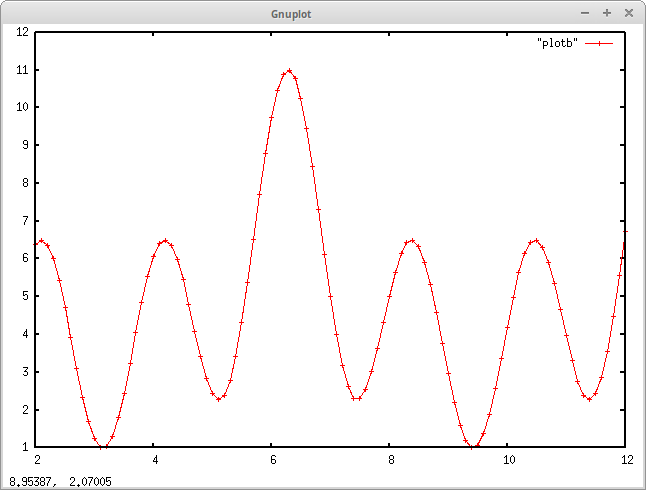
\includegraphics[width=1.00\textwidth]{interpGraph.png}
	\label{fig:interpGraph}
\end{figure}




\end{document}